\documentclass{article}
\usepackage{graphicx} % Required for inserting images
\usepackage[a4paper ,total={7in, 10in}]{geometry}
\title{Using Binomial Trees to map out alternative sports-betting strategies}
\author{Elliott Oates}
\date{April 2024}
\usepackage{setspace}\doublespacing
\usepackage{amsmath}
\usepackage{tikz}
\usetikzlibrary{matrix}
\usepackage[export]{adjustbox}

% Please add the following required packages to your document preamble:
\usepackage{booktabs}
\usepackage{graphicx}

\begin{document}
\pagenumbering{gobble}

The Binomial Option Pricing Model (BOPM), uses risk-neutrality or no-arbitrage conditions to price options via back-propagation based on binary price movements at future stages and is criticized for discrete time frames and binary movements that don't reflect financial markets. These aspects intrigued me a keen sports punter given the discrete nature of scorelines and the binary nature of betting payoffs.

I have devised an algorithm/betting strategy using binomial trees able to replicate outright match bet payoffs through a series of stage-specific, risk-neutral bets that can help punters facing bet-size or betting market access issues. Alternatively, like how trees can determine whether a financial option should be exercised early, it could guide punters with existing outright bets on whether they should exercising the cash out offered. 

Consider a simple example of a punter unable to place a £100 bet for a £200 return on player A winning a 5-set tennis match. Assume each set is independent with a 50\% win probability. The 5 step tree in figure (\ref{fig:scores}) shows the possible set scorelines in the match.\footnote{To simplify the figure, branches that would not be played in a real tennis match are not included}  Player A winning a set would be similar to an 'up' price movement. 

\begin{figure}[h!]
\centering
\caption{Possible Set Scoreline Combinations In a Best of 5 Tennis Match}
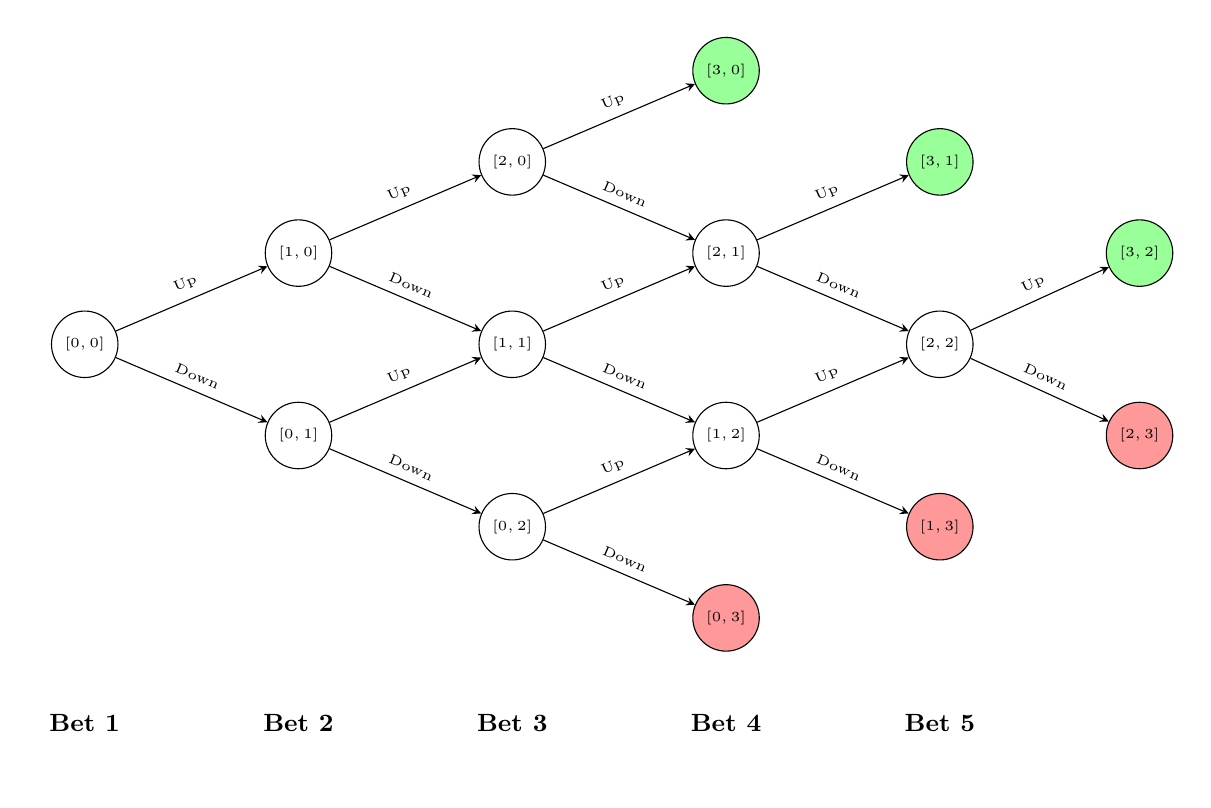
\begin{tikzpicture}[>=stealth,sloped]
    \matrix (tree) [%
        matrix of nodes,
        minimum size=0.8cm,
        column sep=1.5cm,
        row sep=0.3cm,
        nodes={draw, circle, font =\tiny},
    ]
    {  &  &  & |[fill=green!40]|$[3,0]$ &  &   \\ %this is basically a grid, fill in where u need shit
    &  & $[2,0]$ &  &|[fill=green!40]| $[3,1]$ &   \\
    & $[1,0]$ &  & $[2,1]$ &  &|[fill=green!40]| $[3,2]$  \\
    $[0,0]$ &  & $[1,1]$ &  & $[2,2]$ &   \\
    & $[0,1]$ &  & $[1,2]$ &  & |[fill=red!40]|$[2,3]$  \\
    &  & $[0,2]$ & & |[fill=red!40]|$[1,3]$ &   \\
    & & & |[fill=red!40]|$[0,3]$ &  &   \\
    |[draw=none, circle=none, font = \small]|\textbf{Bet 1} &|[draw=none, circle=none, font = \small]| \textbf{Bet 2} & |[draw=none, circle=none, font = \small]|\textbf{Bet 3} & |[draw=none, circle=none, font = \small]|\textbf{Bet 4} & |[draw=none, circle=none, font = \small]|\textbf{Bet 5} &   \\
    };
    \draw[->] (tree-4-1) -- (tree-3-2) node [midway,above] {\tiny Up}; %this is where u put what is on the line between nodes
    \draw[->] (tree-4-1) -- (tree-5-2) node [midway,above] {\tiny Down};
    \draw[->] (tree-3-2) -- (tree-2-3) node [midway,above] {\tiny \tiny Up};
    \draw[->] (tree-3-2) -- (tree-4-3) node [midway,above] {\tiny Down};
    \draw[->] (tree-5-2) -- (tree-4-3) node [midway,above] {\tiny \tiny Up};
    \draw[->] (tree-5-2) -- (tree-6-3) node [midway,above] {\tiny Down};
    \draw[->] (tree-2-3) -- (tree-1-4) node [midway,above] {\tiny \tiny Up};
    \draw[->] (tree-2-3) -- (tree-3-4) node [midway,above] {\tiny Down};
    \draw[->] (tree-4-3) -- (tree-3-4) node [midway,above] {\tiny \tiny Up};
    \draw[->] (tree-4-3) -- (tree-5-4) node [midway,above] {\tiny Down};
    \draw[->] (tree-6-3) -- (tree-5-4) node [midway,above] {\tiny \tiny Up};
    \draw[->] (tree-6-3) -- (tree-7-4) node [midway,above] {\tiny Down};
    \draw[->] (tree-3-4) -- (tree-2-5) node [midway,above] {\tiny \tiny Up};
    \draw[->] (tree-3-4) -- (tree-4-5) node [midway,above] {\tiny Down};
    \draw[->] (tree-5-4) -- (tree-4-5) node [midway,above] {\tiny \tiny Up};
    \draw[->] (tree-5-4) -- (tree-6-5) node [midway,above] {\tiny Down};
    \draw[->] (tree-4-5) -- (tree-3-6) node [midway,above] {\tiny \tiny Up};
    \draw[->] (tree-4-5) -- (tree-5-6) node [midway,above] {\tiny Down};
\end{tikzpicture}
\label{fig:scores}
\end{figure}

At $[2,2]$, a match deciding one has a balance of $X$, and a bet of $Y$ results in a balance of $0$ if player A loses (thus $X=Y$), and a payout of $2Y=200$ if player A wins (making $X = \frac{1}{2}$ the winnings), we find a final bet and balance of £100. By repeating the process for all the nodes where you can infer the same (match deciders) then filling in nodes where you know both possible outcomes one has all the balances and bets at each scoreline as shown in figure (\ref{fig:bets}). 

\begin{figure}
\centering
\caption{Risk Neutral Wagers on Individual Set results that replicate a £100 Match outright Wager }
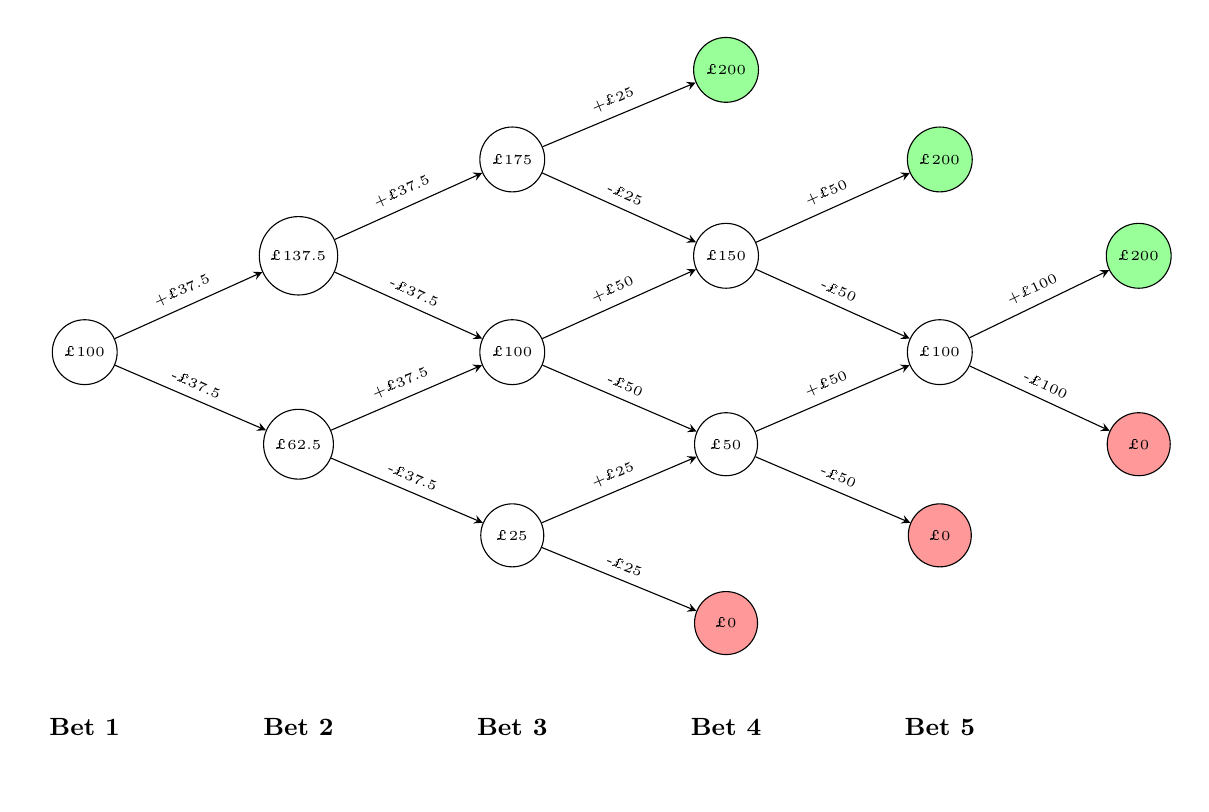
\begin{tikzpicture}[>=stealth,sloped]
    \matrix (tree) [
        matrix of nodes,
        minimum size=0.8cm,
        column sep=1.5cm,
        row sep=0.3cm,
        nodes={draw, circle, font =\tiny},
    ]
    {  &  &  & |[fill=green!40]|£200 &  &   \\
    &  & £175 &  &|[fill=green!40]|£200 &   \\
    & £137.5 &  & £150 &  &|[fill=green!40]|£200  \\
    £100 &  & £100 &  & £100 &   \\
    & £62.5 &  & £50 &  & |[fill=red!40]|£0  \\
    &  & £25 & & |[fill=red!40]|£0 &   \\
    & & & |[fill=red!40]|£0 &  &   \\
    |[draw=none, circle=none, font = \small]|\textbf{Bet 1} &|[draw=none, circle=none, font = \small]| \textbf{Bet 2} & |[draw=none, circle=none, font = \small]|\textbf{Bet 3} & |[draw=none, circle=none, font = \small]|\textbf{Bet 4} & |[draw=none, circle=none, font = \small]|\textbf{Bet 5} &   \\
    };
    \draw[->] (tree-4-1) -- (tree-3-2) node [midway,above] {\tiny +£37.5};
    \draw[->] (tree-4-1) -- (tree-5-2) node [midway,above] {\tiny -£37.5};
    \draw[->] (tree-3-2) -- (tree-2-3) node [midway,above] {\tiny +£37.5};
    \draw[->] (tree-3-2) -- (tree-4-3) node [midway,above] {\tiny -£37.5};
    \draw[->] (tree-5-2) -- (tree-4-3) node [midway,above] {\tiny +£37.5};
    \draw[->] (tree-5-2) -- (tree-6-3) node [midway,above] {\tiny -£37.5};
    \draw[->] (tree-2-3) -- (tree-1-4) node [midway,above] {\tiny +£25};
    \draw[->] (tree-2-3) -- (tree-3-4) node [midway,above] {\tiny -£25};
    \draw[->] (tree-4-3) -- (tree-3-4) node [midway,above] {\tiny +£50};
    \draw[->] (tree-4-3) -- (tree-5-4) node [midway,above] {\tiny -£50};
    \draw[->] (tree-6-3) -- (tree-5-4) node [midway,above] {\tiny +£25};
    \draw[->] (tree-6-3) -- (tree-7-4) node [midway,above] {\tiny -£25};    
    \draw[->] (tree-3-4) -- (tree-2-5) node [midway,above] {\tiny +£50}; 
    \draw[->] (tree-3-4) -- (tree-4-5) node [midway,above] {\tiny -£50};
    \draw[->] (tree-5-4) -- (tree-4-5) node [midway,above] {\tiny +£50};
    \draw[->] (tree-5-4) -- (tree-6-5) node [midway,above] {\tiny -£50};
    \draw[->] (tree-4-5) -- (tree-3-6) node [midway,above] {\tiny +£100};
    \draw[->] (tree-4-5) -- (tree-5-6) node [midway,above] {\tiny -£100};
\end{tikzpicture}
\label{fig:bets}
\end{figure}

While manageable for the tennis match, the above process would get tiresome with baseballs 'best of 7' format and unfeasible with the snooker world championships 'best of 35' format. To produce a general solution/algorithm it was necessary to identify the equivalent option pricing problem. In the tennis case we have a digital option that pays +£100 if A wins 3 or more sets and -100£ otherwise and the underlying asset simply is a random walk that goes up or down at each state. 

For the general case of a match that is best of $T$ sets where player A needs $S = \frac{T+1}{2}$ wins, the wager at node $[i,j]$ equals half (if betting at evens) the value difference between child nodes $[i+1,j]$ (up state) and $[i,j+1]$ (down state). 

The value in the up state $[i+1,j]$ is given by the probability of winning $S-i-1$ or more of the remaining $T-i-j-1$ sets minus the probability of winning $S-i-2$ or fewer out of the remaining\footnote{Since sets are discrete, $S-i-2$ or fewer $\equiv$ less than $S-i$. Therefore $P(X\leq k-1)$ and $P(X < k)$ are interchangeable}. Conversely, the value in the down state $[i,j+1]$ is given by the probability winning $S-i$ or more of the remaining $T-i-j-1$ sets minus the probability of winning $S-i-1$ or fewer out of the remaining.

The general formula for the probability of winning at least $k$ more sets out of the $n$ remaining is given by: 
\[
P(X \geq k) = \sum_{l=k}^{n} \binom{n}{l} p^l (1-p)^{n-l}
\]

where $\binom{n}{l} = \frac{n!}{l!(n-l)!}$, and $P(X < k) = 1 - P(X\geq k)$.

For an initial balance of £100, values $V_u$ and $V_d$ as: 
\[V_u = 100 \times P(X \geq S-i-1) - 100 \times(1-P(X \geq S -i-1) \]
\[V_d = 100 \times P(X \geq S-i) - 100\times(1-P(X \geq S -i)) \]

Thus, the wager, $W_{i,j}$, is: \[ W_{i,j} = \frac{1}{2}(V_u - V_d) \]

While the process holds at terminal nodes, it fails when $i=j$, i.e. the deciding set but this is intuitively just the original outright wager. 

Referring back to the tennis example the initial wager when the score is $[0,0]$ is derived as follows. 
\[ P(X \geq 2) = \sum_{l=2}^{4}\binom{4}{l}\left(\frac{1}{2}\right)^{l}\left(1-\frac{1}{2}\right)^{4-l} = 0.6875\]
\[ P(X \geq 3) = \sum_{l=3}^{4}\binom{4}{l}\left(\frac{1}{2}\right)^{l}\left(1-\frac{1}{2}\right)^{4-l} = 0.3125\]

$V_u$ and $V_d$ are £37.5 and -£37.5 therefore, the first set wager $W_{0,0}$ is £37.5, reflecting symmetric probabilities when scorelines are tied.
 
\begin{table}[h!]
\centering
\caption{Proof of concept applied to other stages in a 5 set match}
\label{tab:my-table}
\resizebox{\columnwidth}{!}{%
\begin{tabular}{ccccccc}
\hline
\textbf{\begin{tabular}[c]{@{}c@{}}Scoreline\\ (Node)\end{tabular}} &
  \textbf{\begin{tabular}[c]{@{}c@{}}Sets Remaining\\ At Child Nodes\end{tabular}} &
  \textbf{$P(X\geq S - i - 1)$} &
  \textbf{$V_u$} &
  \textbf{$P(X\geq S - i)$} &
  \textbf{$V_d$} &
  \textbf{\begin{tabular}[c]{@{}c@{}}Wager\\ $W_{i,j}$\end{tabular}} \\ \hline
{[}0,0{]} & 4 & 0.6875 & £37.5 & 0.3125 & £31.25 & £37.5 \\
{[}0,1{]} & 3 & 0.125  & 0     & 0.125  & -£75   & £37.5 \\
{[}2,0{]} & 2 & 1      & £100  & 0.75   & £50    & £25   \\
{[}2,1{]} & 1 & 1      & £100  & 0.5    & £0     & £50   \\ \hline
\end{tabular}%
}
\end{table}

\begin{figure}[b!]
    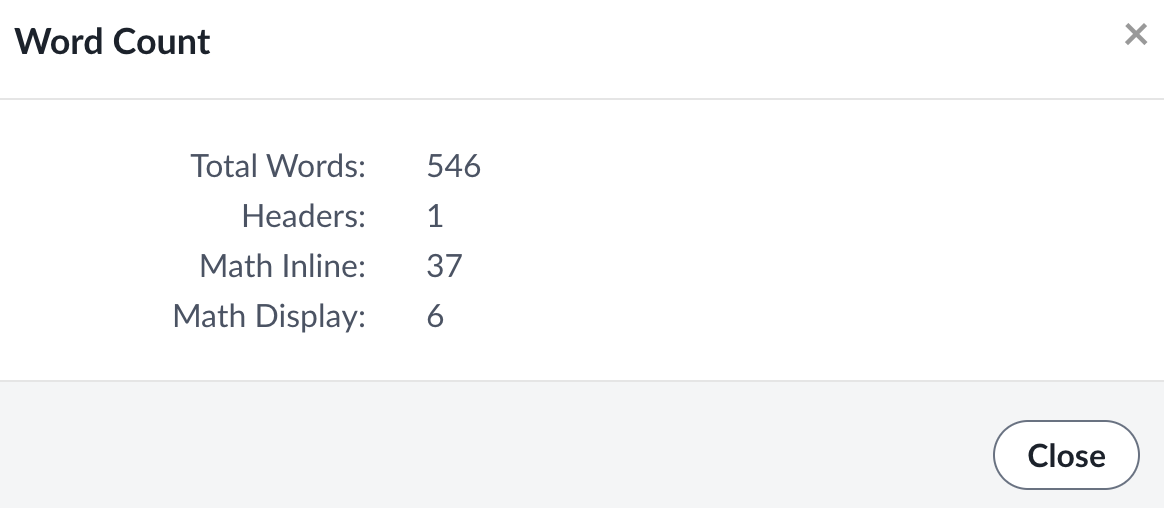
\includegraphics[width=0.5\linewidth,left]{image.png}
    \label{fig:enter-label}
\end{figure}

\end{document}